\documentclass[12pt]{article}
\usepackage[english]{babel}
\usepackage{natbib}
\usepackage{url}
\usepackage[utf8x]{inputenc}
\usepackage{amsmath}
\usepackage{graphicx}
\graphicspath{{images/}}
\usepackage{parskip}
\usepackage{fancyhdr}
\usepackage{vmargin}
\usepackage{xcolor}
\usepackage{siunitx}
\usepackage{physics}
\setmarginsrb{3 cm}{2 cm}{3 cm}{2 cm}{1 cm}{1.5 cm}{1 cm}{1.5 cm}

\title{Lab 08}													% Title
\author{G 03}														% Author
\date{28 may 2019}														% Date

\makeatletter
\let\thetitle\@title
\let\theauthor\@author
\let\thedate\@date
\makeatother

\pagestyle{fancy}
\fancyhf{}
\rhead{\theauthor}
\lhead{\thetitle}
\cfoot{\thepage}
\newcommand{\mis}[3]{(#1 \pm #2) \ #3}
\newcommand{\misp}[3]{(#1 \#3 \pm #2}
\begin{document}

%%%%%%%%%%%%%%%%%%%%%%%%%%%%%%%%%%%%%%%%%%%%%%%%%%%%%%%%%%%%%%%%%%%%%%%%%%%%%%%%%%%%%%%%%

\begin{titlepage}
	\centering
    \vspace*{0.5 cm}
    
\includegraphics[scale = 0.75]{polito.jpg}\\[1.0 cm]				% University Logo
    \textsc{\LARGE Politecnico di Torino}\\[2.0 cm]						% University Name
	\textsc{\Large Digital systems electronics\\ A.A. 2018/2019}\\[0.5 cm]		% Course Code
	\textsc{\Large Prof. G. Masera}\\[0.5 cm]		% Nome del Professore
	\rule{\linewidth}{0.2 mm} \\[0.4 cm]
	{ \huge \bfseries \thetitle \\ \small \thedate}\\
	\rule{\linewidth}{0.2 mm} \\[1.5 cm]
	
	\begin{minipage}{0.4\textwidth}
		\begin{flushleft} \large
			Berchialla Luca\\												%Cognomi e nomi
			Laurasi Gjergji
			\\
			
			Mattei Andrea\\
            Lombardo Domenico Maria\\
            Wylezek Karolina
            
			\end{flushleft}
			\end{minipage}~
			\begin{minipage}{0.4\textwidth}
            
			\begin{flushright} \large
			236032\\													%Matricole
			238259\\
            233755\\
            233959\\
            267219\\
            
		\end{flushright}
        
	\end{minipage}\\[2 cm]
	
\end{titlepage}

%%%%%%%%%%%%%%%%%%%%%%%%%%%%%%%%%%%%%%%%%%%%%%%%%%%%%%%%%%%%%%%%%%%%%%%%%%%%%%%%%%%%%%%%%
\newpage

\section*{Output compare VS Reload}
{
	
	In the following report the Output Compare register and/or auto-reload register can be calculated from the desired asserted flag frequency using the following formula:
	\[F_{X}=\frac{F_{CLK}}{(OC+1)\cdot(ARR+1)}\;\;\;\;\; (1)\] 
	
	Notice that to correctly generate a square wave with a desired frequency $F_{X}$ exploiting the OC or ARR approach, the formula 1 should also be divided by a 2 factor.
}

\section*{1.1 }
Following the instructions on the lab8 document we created the project with cube mx, where just had to set the auto reload register to the proper value calculated with the formula mentioned before.\\
In the source code we polled the counter register to a random integer smaller or equal than the ARR value to toggle the output pin (in our code we used the arr value). \\
With the oscilloscope we can clearly see that this approach doesn't work because just a few times the MCU is detecting that the counter register and our random integer are equal. Instead when we use the condition $"counter<=arr"$ the pin is toggled every time that the MCU executes it, therefor we observed a frequency of 1.6 MHz.

\begin{figure}[h!]
	
	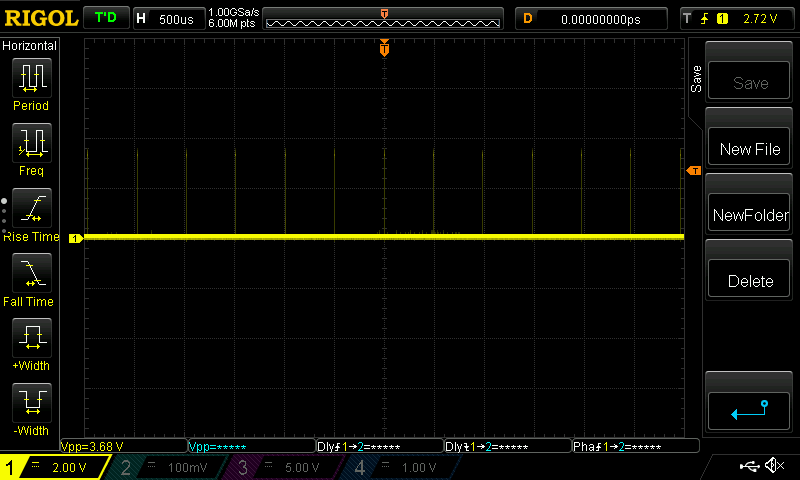
\includegraphics[scale = 0.4]{immagini/NewFile1}
	\caption{condition $"counter=arr"$ }
\end{figure}

\begin{figure}[h!]
	
	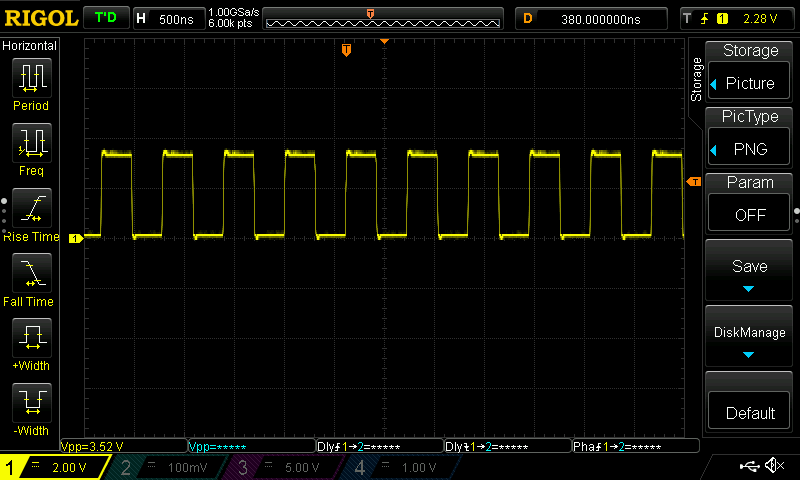
\includegraphics[scale = 0.4]{immagini/DS1Z_QuickPrint1}
	\caption{condition $"counter<=arr"$ }
\end{figure}



\section*{1.2 }
In this section we reused the code of the previous point but this time we polled the auto reload register flag.\\
\begin{figure}[h!]
	
	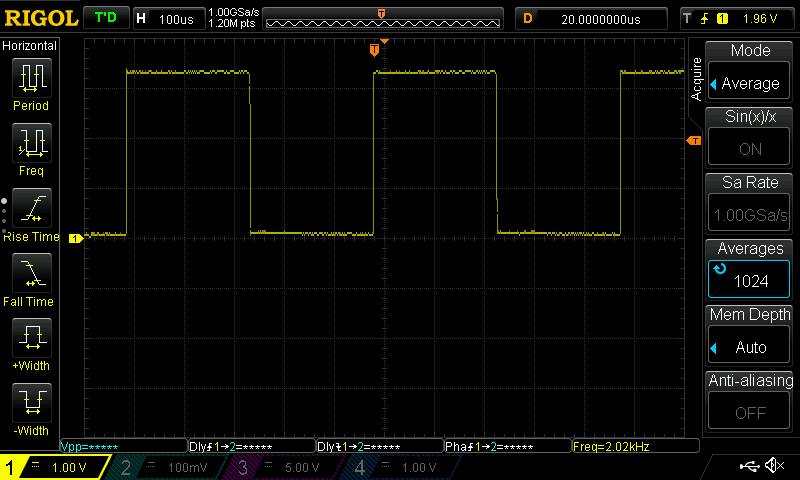
\includegraphics[scale = 0.4]{immagini/DS1Z_QuickPrint4}
	\caption{2 kHz wave }
\end{figure}
If we try to achieve 4 MHz we can see that the board can't deliver such a high frequency, actually we registered 1.6 MHz. 
\begin{figure}[h!]
	
	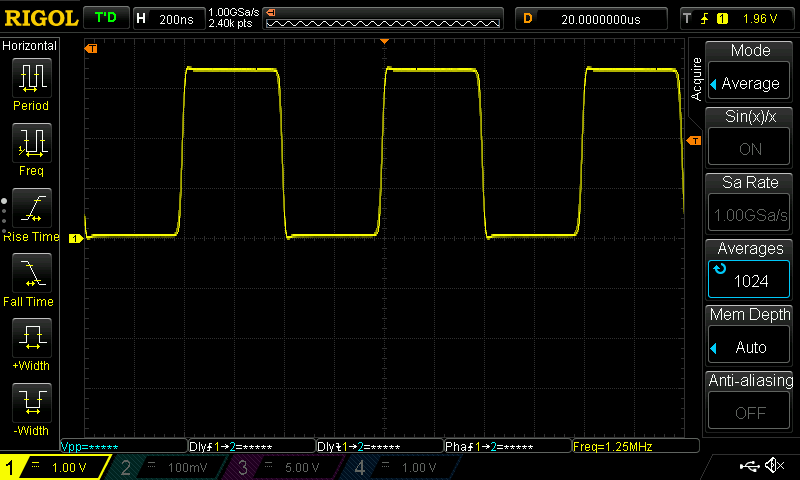
\includegraphics[scale = 0.4]{immagini/DS1Z_QuickPrint3}
	\caption{should be 4Mhz wave }
\end{figure}


\section*{1.3}
In this section we had to use the capture compare unit in order to generate the square wave, to use this approach we have to let the counter count up to its maximum value. To generate the wave we use the flag generated by the capture compare unit. The capture compare register is incremented every time we detect the flag in order to have an event every half period. The value of the increment is calculated with the formula mentioned before.
\begin{figure}[h!]
	
	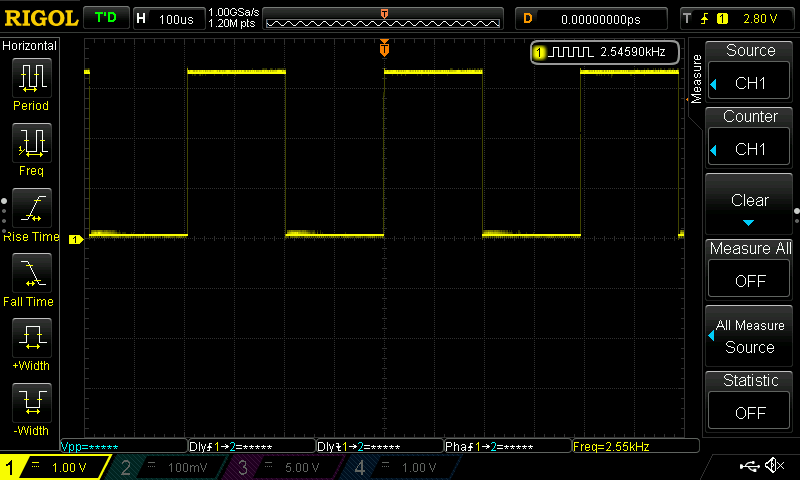
\includegraphics[scale = 0.4]{immagini/DS1Z_QuickPrint6}
	\caption{should be 4Mhz wave }
\end{figure}


\section*{1.4 }
image 7 e 9

800 Hz \space $->$ oc register: 531\\
1.2 kHz $->$ oc register: 353\\
3.0 kHz $->$ oc register: 142\\
4.5 kHz $->$ oc register: 95\\


\end{document}




